\documentclass[11pt]{article}

\usepackage[margin=1in]{geometry}
\usepackage[T1]{fontenc}
\usepackage[utf8]{inputenc}
\usepackage{lmodern}
\usepackage{microtype}
\usepackage{amsmath,amssymb,amsthm,mathtools}
\usepackage{bm}
\usepackage{booktabs,array,longtable,multirow}
\usepackage{hyperref}
\usepackage{xcolor}
\usepackage[most]{tcolorbox}
\usepackage{tikz}
\usepackage{pgfplots}
\usepackage{pgfplotstable}
\usepackage{tikz-3dplot}
\usepackage{enumitem}
\usepackage{caption}
\usepackage{float}
\usepackage{fancyhdr}
\usepackage{titlesec}

\pgfplotsset{compat=1.18}
\usepgfplotslibrary{fillbetween}
\usetikzlibrary{arrows.meta,calc,intersections,patterns,decorations.pathreplacing,positioning,3d,backgrounds,matrix}

\hypersetup{
  colorlinks=true,
  linkcolor=blue!60!black,
  urlcolor=blue!60!black,
  citecolor=blue!60!black,
  pdftitle={Chapter 8. Partial Derivatives and the Gradient}
}

\setlength{\headheight}{14pt}
\setlength{\parindent}{0pt}
\setlength{\parskip}{0.65em}
\setlist[itemize]{topsep=2pt,itemsep=2pt}
\setlist[enumerate]{topsep=2pt,itemsep=2pt}

\titleformat{\section}{\large\bfseries}{\thesection}{0.6em}{}
\titleformat{\subsection}{\normalsize\bfseries}{\thesubsection}{0.6em}{}

\pagestyle{fancy}
\fancyhf{}
\lhead{Chapter 8. Partial Derivatives and the Gradient}
\rhead{\thepage}
\renewcommand{\headrulewidth}{0.4pt}

\newtcolorbox{chapteroverviewbox}{
  colback=blue!4,
  colframe=blue!50!black,
  boxrule=0.7pt,
  arc=2mm,
  left=2mm,right=2mm,top=1mm,bottom=1mm
}

\newtcolorbox{goalbox}{
  colback=green!4,
  colframe=green!45!black,
  title=Learning goals,
  fonttitle=\bfseries,
  boxrule=0.7pt,
  arc=2mm
}

\newtcolorbox{notebox}[1][]{
  colback=blue!3,
  colframe=blue!50!black,
  fonttitle=\bfseries,
  title=#1,
  boxrule=0.7pt,
  arc=2mm
}

\newtcolorbox{tipbox}[1][]{
  colback=green!3,
  colframe=green!45!black,
  fonttitle=\bfseries,
  title=#1,
  boxrule=0.7pt,
  arc=2mm
}

\newtcolorbox{importantbox}[1][]{
  colback=red!3,
  colframe=red!60!black,
  fonttitle=\bfseries,
  title=#1,
  boxrule=0.7pt,
  arc=2mm
}

\newtcolorbox{warningbox}[1][]{
  colback=yellow!8,
  colframe=orange!75!black,
  fonttitle=\bfseries,
  title=#1,
  boxrule=0.7pt,
  arc=2mm
}

\newtcbtheorem[number within=section]{examplebox}{Example}{
  enhanced,
  breakable,
  colback=white,
  colframe=blue!60!black,
  colbacktitle=blue!60!black,
  fonttitle=\bfseries,
  boxrule=0.7pt,
  arc=1.5mm,
  left=2mm,right=2mm,top=1mm,bottom=1mm
}{ex}

\newcommand{\R}{\mathbb R}
\newcommand{\grad}{\nabla}
\newcommand{\dd}{\,d}
\newcommand{\ii}{\mathbf i}
\newcommand{\jj}{\mathbf j}

\begin{document}

\begin{center}
  {\LARGE\bfseries Chapter 8. Partial Derivatives and the Gradient\par}
  \vspace{0.3em}
  {\large Coordinate rates of change, sensitivity, and local information\par}
\end{center}

\begin{chapteroverviewbox}
A function of one variable has one basic input direction: move left or move right on the number line. A function of several variables has many input directions. The first step is to measure change in coordinate directions.

For a function $f(x,y)$, the partial derivative $f_x$ measures the instantaneous rate of change when $x$ changes and $y$ is held fixed. The partial derivative $f_y$ measures the instantaneous rate of change when $y$ changes and $x$ is held fixed. Together they form the \emph{gradient vector}
\[
\grad f(x,y)=\langle f_x(x,y),f_y(x,y)\rangle.
\]
The gradient is the local direction-information vector for a scalar field. It tells us how the output changes to first order near a point, how level curves are oriented, and how a loss function changes when model parameters change.
\end{chapteroverviewbox}

\begin{notebox}[Teaching-material connection]
This chapter develops the material on partial derivatives, geometric traces, numerical derivative estimates, second partial derivatives, Clairaut's theorem, and the gradient vector. The main idea is that partial derivatives reduce multivariable differentiation to single-variable differentiation by holding all other variables fixed.
\end{notebox}

\begin{goalbox}
After studying this chapter, you should be able to:
\begin{enumerate}
  \item define $f_x(a,b)$ and $f_y(a,b)$ using limits;
  \item interpret partial derivatives as slopes of coordinate traces of a surface;
  \item compute partial derivatives by treating other variables as constants;
  \item estimate partial derivatives from data or finite differences;
  \item compute second partial derivatives and mixed partial derivatives;
  \item use Clairaut's theorem when mixed partial derivatives are continuous;
  \item compute the gradient of functions on $\R^2$, $\R^3$, and $\R^n$;
  \item explain why the gradient is perpendicular to level curves and level surfaces;
  \item connect gradients with sensitivity analysis, image processing, statistics, and machine learning.
\end{enumerate}
\end{goalbox}

\section{From one derivative to many partial derivatives}

For a single-variable function $y=f(x)$, the derivative at $x=a$ is
\[
f'(a)=\lim_{h\to 0}\frac{f(a+h)-f(a)}{h}.
\]
Geometrically, this is the slope of the tangent line at $x=a$. For a two-variable function $z=f(x,y)$, the graph is a surface. At a point $(a,b,f(a,b))$, there are many possible curves on the surface passing through that point. The easiest ones are the two coordinate traces:
\begin{itemize}
  \item the trace obtained by fixing $y=b$ and allowing $x$ to vary;
  \item the trace obtained by fixing $x=a$ and allowing $y$ to vary.
\end{itemize}
The slopes of these traces are the partial derivatives.

\begin{importantbox}[Core idea]
A partial derivative is an ordinary derivative applied to a slice of a multivariable function.
\end{importantbox}

\section{Definitions of $f_x$ and $f_y$}

Let $f$ be a function of two variables. The partial derivative of $f$ with respect to $x$ at $(a,b)$ is
\[
f_x(a,b)=\lim_{h\to 0}\frac{f(a+h,b)-f(a,b)}{h},
\]
provided the limit exists. The partial derivative of $f$ with respect to $y$ at $(a,b)$ is
\[
f_y(a,b)=\lim_{h\to 0}\frac{f(a,b+h)-f(a,b)}{h},
\]
provided the limit exists.

Equivalently, if $g(x)=f(x,b)$, then $f_x(a,b)=g'(a)$. If $k(y)=f(a,y)$, then $f_y(a,b)=k'(b)$.

The notation is flexible:
\[
f_x=\frac{\partial f}{\partial x}=\frac{\partial z}{\partial x}=D_x f,
\qquad
f_y=\frac{\partial f}{\partial y}=\frac{\partial z}{\partial y}=D_y f.
\]

\begin{tipbox}[How to compute partial derivatives]
To compute $f_x$, treat $y$ as a constant and differentiate with respect to $x$. To compute $f_y$, treat $x$ as a constant and differentiate with respect to $y$.
\end{tipbox}

\section{Geometric interpretation: slopes of traces}

Suppose the surface is $z=f(x,y)$ and we focus on the point $(a,b,f(a,b))$. The trace in the plane $y=b$ is the single-variable curve $z=f(x,b)$. Its tangent slope at $x=a$ is $f_x(a,b)$. The trace in the plane $x=a$ is $z=f(a,y)$, and its tangent slope at $y=b$ is $f_y(a,b)$.

\begin{examplebox}{A surface and its coordinate traces}{surftraces}
Let
\[
f(x,y)=4-\frac{x^2}{4}-y^2.
\]
This is a downward-opening elliptic paraboloid. At the point $(1,1)$,
\[
f_x(x,y)=-\frac{x}{2},\qquad f_y(x,y)=-2y.
\]
Thus
\[
f_x(1,1)=-\frac12,\qquad f_y(1,1)=-2.
\]
Interpretation:
\begin{itemize}
  \item if $y=1$ is held fixed and $x$ increases near $x=1$, the height decreases at rate $1/2$;
  \item if $x=1$ is held fixed and $y$ increases near $y=1$, the height decreases at rate $2$.
\end{itemize}
\end{examplebox}

\begin{figure}[H]
\centering
\begin{tikzpicture}
\begin{axis}[
  width=0.78\textwidth,
  view={60}{26},
  xlabel={$x$},ylabel={$y$},zlabel={$z$},
  domain=-4:4, y domain=-2.2:2.2,
  samples=28,samples y=22,
  colormap/viridis,
  z buffer=sort,
  title={Surface with coordinate traces}
]
\addplot3[surf,opacity=0.7,shader=interp] {4 - x^2/4 - y^2};
\addplot3[very thick,red!80!black,domain=-4:4,samples=150] ({x},{1},{4 - x^2/4 - 1});
\addplot3[very thick,blue!80!black,domain=-2.2:2.2,samples=150] ({1},{x},{4 - 1/4 - x^2});
\addplot3[only marks,mark=*,mark size=2.2pt] coordinates {(1,1,2.75)};
\end{axis}
\end{tikzpicture}
\caption{Coordinate traces of $f(x,y)=4-x^2/4-y^2$ through the point $(1,1,2.75)$. The partial derivatives are the slopes of these traces.}
\end{figure}

\section{Computing partial derivatives}

\begin{examplebox}{Polynomial, trigonometric, and exponential terms}{polytrigexp}
Let
\[
f(x,y)=x^3+x^2\sin y-xe^y.
\]
To compute $f_x$, hold $y$ constant:
\[
f_x(x,y)=3x^2+2x\sin y-e^y.
\]
To compute $f_y$, hold $x$ constant:
\[
f_y(x,y)=x^2\cos y-xe^y.
\]
At $(1,2)$,
\[
f_x(1,2)=3+2\sin 2-e^2,
\qquad
f_y(1,2)=\cos 2-e^2.
\]
\end{examplebox}

\begin{examplebox}{A radial function}{radialf}
Let
\[
f(x,y)=\sqrt{x^2+y^2}.
\]
For $(x,y)\ne(0,0)$,
\[
f_x(x,y)=\frac{x}{\sqrt{x^2+y^2}},
\qquad
f_y(x,y)=\frac{y}{\sqrt{x^2+y^2}}.
\]
At $(1,2)$,
\[
f_x(1,2)=\frac{1}{\sqrt5},\qquad f_y(1,2)=\frac{2}{\sqrt5}.
\]
At the origin, these formulas do not apply because the denominator vanishes. In fact, $f_x(0,0)$ and $f_y(0,0)$ exist, but the function is not differentiable there. Partial derivatives give coordinate-direction information, but not always the whole story.
\end{examplebox}

\section{Partial derivatives from data}

In applications, we often do not know a symbolic formula for $f$. We may only have sampled values. Then partial derivatives are estimated by finite differences. For example,
\[
f_x(1,2)\approx \frac{f(1.1,2)-f(1,2)}{0.1},
\qquad
f_y(1,2)\approx \frac{f(1,2.15)-f(1,2)}{0.15}.
\]
This idea is fundamental in numerical differentiation, image processing, computer vision, and machine learning.

\begin{examplebox}{Finite-difference estimates}{fdest}
For $f(x,y)=x^3+x^2\sin y-xe^y$, forward differences provide simple estimates for $f_x(1,2)$ and $f_y(1,2)$. A more accurate approximation often uses centered differences:
\[
f_x(a,b)\approx \frac{f(a+h,b)-f(a-h,b)}{2h}.
\]
The same idea works for $f_y$.
\end{examplebox}

\begin{figure}[H]
\centering
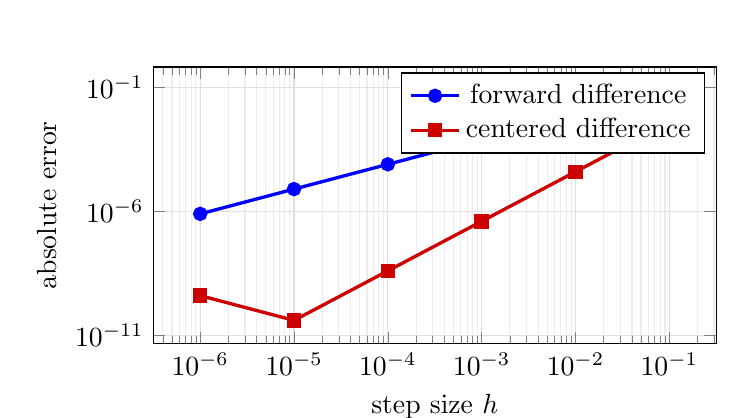
\begin{tikzpicture}
\begin{loglogaxis}[
  width=0.72\textwidth,
  height=0.42\textwidth,
  xlabel={step size $h$},
  ylabel={absolute error},
  legend style={at={(0.98,0.98)},anchor=north east,fill=white},
  grid=both,
  minor grid style={gray!15},
  major grid style={gray!25}
]
\addplot[very thick,mark=*,blue] coordinates {
(1e-1,8e-2) (1e-2,8e-3) (1e-3,8e-4) (1e-4,8e-5) (1e-5,8e-6) (1e-6,8e-7)};
\addlegendentry{forward difference}
\addplot[very thick,mark=square*,red!80!black] coordinates {
(1e-1,4e-3) (1e-2,4e-5) (1e-3,4e-7) (1e-4,4e-9) (1e-5,4e-11) (1e-6,4e-10)};
\addlegendentry{centered difference}
\end{loglogaxis}
\end{tikzpicture}
\caption{Centered differences usually converge faster than forward differences for smooth functions. The red curve drops more rapidly as $h$ decreases.}
\end{figure}

\section{Image processing interpretation}

An image can be viewed as a function
\[
I(x,y)=\text{pixel intensity at location }(x,y).
\]
Then $I_x$ measures horizontal change and $I_y$ measures vertical change. Large values of $|I_x|$ or $|I_y|$ often indicate edges. This is the same calculus idea, but applied to a matrix of data instead of a symbolic formula.

\begin{figure}[H]
\centering
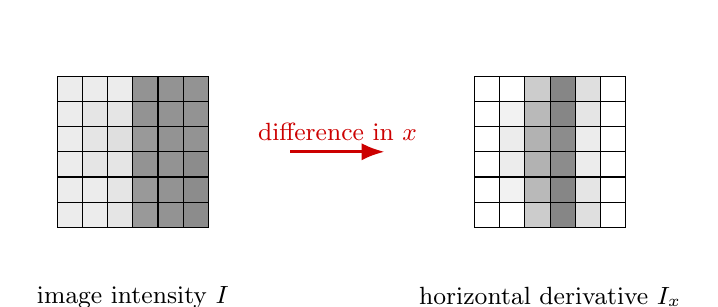
\begin{tikzpicture}[font=\small]
  \matrix[matrix of nodes,nodes={draw,minimum size=0.32cm,inner sep=0pt,anchor=center},column sep=-\pgflinewidth,row sep=-\pgflinewidth] (A) at (0,0) {
  |[fill=gray!15]| & |[fill=gray!15]| & |[fill=gray!15]| & |[fill=gray!85]| & |[fill=gray!85]| & |[fill=gray!85]| \\
  |[fill=gray!15]| & |[fill=gray!20]| & |[fill=gray!20]| & |[fill=gray!85]| & |[fill=gray!85]| & |[fill=gray!85]| \\
  |[fill=gray!15]| & |[fill=gray!20]| & |[fill=gray!25]| & |[fill=gray!80]| & |[fill=gray!85]| & |[fill=gray!85]| \\
  |[fill=gray!15]| & |[fill=gray!20]| & |[fill=gray!20]| & |[fill=gray!85]| & |[fill=gray!85]| & |[fill=gray!90]| \\
  |[fill=gray!15]| & |[fill=gray!15]| & |[fill=gray!20]| & |[fill=gray!80]| & |[fill=gray!85]| & |[fill=gray!90]| \\
  |[fill=gray!15]| & |[fill=gray!15]| & |[fill=gray!20]| & |[fill=gray!80]| & |[fill=gray!85]| & |[fill=gray!90]| \\
  };
  \node[below=0.5cm of A] {image intensity $I$};

  \matrix[matrix of nodes,nodes={draw,minimum size=0.32cm,inner sep=0pt,anchor=center},column sep=-\pgflinewidth,row sep=-\pgflinewidth] (B) at (5.3,0) {
  |[fill=white]| & |[fill=white]| & |[fill=gray!40]| & |[fill=gray!95]| & |[fill=gray!25]| & |[fill=white]| \\
  |[fill=white]| & |[fill=gray!10]| & |[fill=gray!55]| & |[fill=gray!95]| & |[fill=gray!20]| & |[fill=white]| \\
  |[fill=white]| & |[fill=gray!15]| & |[fill=gray!60]| & |[fill=gray!90]| & |[fill=gray!15]| & |[fill=white]| \\
  |[fill=white]| & |[fill=gray!15]| & |[fill=gray!60]| & |[fill=gray!90]| & |[fill=gray!15]| & |[fill=white]| \\
  |[fill=white]| & |[fill=gray!10]| & |[fill=gray!55]| & |[fill=gray!95]| & |[fill=gray!20]| & |[fill=white]| \\
  |[fill=white]| & |[fill=white]| & |[fill=gray!40]| & |[fill=gray!95]| & |[fill=gray!25]| & |[fill=white]| \\
  };
  \node[below=0.5cm of B] {horizontal derivative $I_x$};
  \draw[very thick,red!80!black,-Latex] (2.0,0) -- (3.2,0) node[midway,above] {difference in $x$};
\end{tikzpicture}
\caption{Finite differences applied to image-like data. Horizontal derivatives reveal sharp transitions, which are often edges.}
\end{figure}

\begin{notebox}[Modern interpretation]
In symbolic calculus, $f_x$ and $f_y$ are formulas. In data analysis, they are often approximations computed from samples, grids, or pixels. The concept is the same: measure local change in coordinate directions.
\end{notebox}

\section{Second partial derivatives}

If $z=f(x,y)$, then the four second partial derivatives are
\[
f_{xx}=\frac{\partial}{\partial x}\left(\frac{\partial f}{\partial x}\right),
\qquad
f_{xy}=\frac{\partial}{\partial y}\left(\frac{\partial f}{\partial x}\right),
\]
\[
f_{yx}=\frac{\partial}{\partial x}\left(\frac{\partial f}{\partial y}\right),
\qquad
f_{yy}=\frac{\partial}{\partial y}\left(\frac{\partial f}{\partial y}\right).
\]
The derivatives $f_{xy}$ and $f_{yx}$ are the \emph{mixed partial derivatives}.

\begin{examplebox}{Second partials and mixed partials}{mixedpartials}
Let
\[
f(x,y)=x^2+xy^3+\sin(xy).
\]
First derivatives:
\[
f_x=2x+y^3+y\cos(xy),
\qquad
f_y=3xy^2+x\cos(xy).
\]
Second derivatives:
\[
f_{xx}=2-y^2\sin(xy),
\]
\[
f_{xy}=3y^2+\cos(xy)-xy\sin(xy),
\]
\[
f_{yx}=3y^2+\cos(xy)-xy\sin(xy),
\]
\[
f_{yy}=6xy-x^2\sin(xy).
\]
Here the mixed partial derivatives are equal.
\end{examplebox}

\section{Clairaut's theorem}

\begin{importantbox}[Clairaut's theorem]
Suppose $f$ is defined on a disk containing $(a,b)$. If $f_{xy}$ and $f_{yx}$ are both continuous on that disk, then
\[
f_{xy}(a,b)=f_{yx}(a,b).
\]
\end{importantbox}

In most elementary examples involving polynomials, exponentials, logarithms, and trigonometric functions on regions where the formulas are defined, the continuity hypothesis is satisfied. Then the order of mixed partial differentiation can be switched.

\section{The gradient vector}

The first partial derivatives form a vector. For $f(x,y)$,
\[
\grad f(x,y)=\langle f_x(x,y),f_y(x,y)\rangle.
\]
For $f(x,y,z)$,
\[
\grad f(x,y,z)=\langle f_x(x,y,z),f_y(x,y,z),f_z(x,y,z)\rangle.
\]
More generally, for $f(x_1,\ldots,x_n)$,
\[
\grad f(x_1,\ldots,x_n)=\left\langle
\frac{\partial f}{\partial x_1},
\frac{\partial f}{\partial x_2},
\ldots,
\frac{\partial f}{\partial x_n}
\right\rangle.
\]
The symbol $\nabla$ is pronounced \emph{del} or \emph{nabla}.

\begin{examplebox}{Gradient of a two-variable function}{grad2var}
Let
\[
f(x,y)=\sin(xy)+e^y.
\]
Then
\[
f_x=y\cos(xy),
\qquad
f_y=x\cos(xy)+e^y.
\]
Therefore
\[
\grad f(x,y)=\langle y\cos(xy),x\cos(xy)+e^y\rangle.
\]
At $(0,1)$,
\[
\grad f(0,1)=\langle 1,e\rangle.
\]
\end{examplebox}

\begin{examplebox}{Gradient of a three-variable function}{grad3var}
Let
\[
f(x,y,z)=xyz.
\]
Then
\[
f_x=yz,\qquad f_y=xz,\qquad f_z=xy.
\]
Thus
\[
\grad f(x,y,z)=\langle yz,xz,xy\rangle.
\]
At $(1,2,3)$,
\[
\grad f(1,2,3)=\langle 6,3,2\rangle.
\]
\end{examplebox}

\section{The gradient and level curves}

Level curves have equations $f(x,y)=c$. The gradient $\grad f$ is perpendicular to the level curve at points where $\grad f\ne 0$.

Suppose $r(t)=\langle x(t),y(t)\rangle$ is a curve that stays on the level curve $f(x,y)=c$. Then $f(x(t),y(t))=c$. Differentiating gives
\[
\grad f(x(t),y(t))\cdot r'(t)=0.
\]
The vector $r'(t)$ is tangent to the level curve. Therefore the gradient is perpendicular to the tangent direction.

\begin{importantbox}[Geometric meaning of the gradient]
The gradient points normal to level curves and level surfaces. It tells us which direction cuts most directly across the contours.
\end{importantbox}

\begin{figure}[H]
\centering
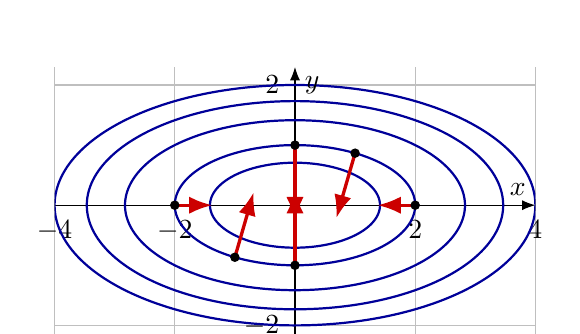
\begin{tikzpicture}
\begin{axis}[
  width=0.68\textwidth,
  height=0.42\textwidth,
  xmin=-4,xmax=4,
  ymin=-2.3,ymax=2.3,
  axis equal image,
  axis lines=middle,
  xlabel={$x$},ylabel={$y$},
  grid=both,
  axis line style={-Latex}
]
\foreach \c in {0,1,2,3,3.5}{
  \pgfmathsetmacro{\yr}{sqrt(max(0,4-\c))}
  \pgfmathsetmacro{\xr}{2*sqrt(max(0,4-\c))}
  \addplot[domain=0:360,samples=220,blue!60!black,thick] ({\xr*cos(x)},{\yr*sin(x)});
}
\foreach \px/\py/\ux/\vy in {2/0/-1/0,-2/0/1/0,0/1/0/-2,0/-1/0/2,1/0.866/-0.5/-1.732,-1/-0.866/0.5/1.732}{
  \pgfmathsetmacro{\qx}{\px+\ux/1.6}
  \pgfmathsetmacro{\qy}{\py+\vy/1.6}
  \addplot[only marks,mark=*,mark size=1.5pt] coordinates {(\px,\py)};
  \addplot[red!80!black,very thick,-Latex] coordinates {(\px,\py) (\qx,\qy)};
}
\end{axis}
\end{tikzpicture}
\caption{Gradient vectors are perpendicular to level curves of $H(x,y)=4-x^2/4-y^2$.}
\end{figure}

\section{Gradient fields}

For each point $(x,y)$, the gradient produces a vector $\grad f(x,y)$. The collection of these vectors is called a \emph{gradient field}. Gradient fields show local directions of increase and form an important special class of vector fields.

\begin{figure}[H]
\centering
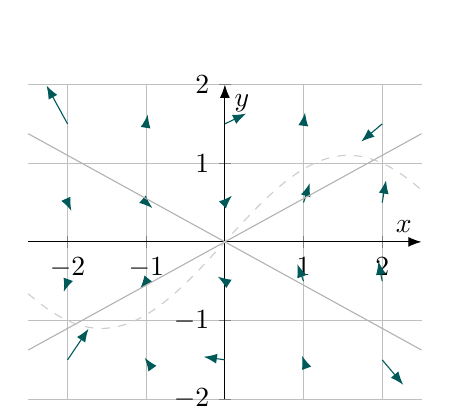
\begin{tikzpicture}
\begin{axis}[
  width=0.72\textwidth,
  height=0.46\textwidth,
  xmin=-2.5,xmax=2.5,
  ymin=-2,ymax=2,
  axis equal image,
  axis lines=middle,
  xlabel={$x$},ylabel={$y$},
  grid=both,
  axis line style={-Latex}
]
\foreach \a in {-2,-1,0,1,2}{
  \foreach \b in {-1.5,-0.5,0.5,1.5}{
    \pgfmathsetmacro{\fx}{\b*cos(deg(\a*\b))}
    \pgfmathsetmacro{\fy}{\a*cos(deg(\a*\b)) + 0.4*exp(0.4*\b)}
    \pgfmathsetmacro{\axend}{\a+0.18*\fx}
    \pgfmathsetmacro{\ayend}{\b+0.18*\fy}
    \addplot[teal!70!black,-Latex] coordinates {(\a,\b) (\axend,\ayend)};
  }
}
\addplot[domain=-2.5:2.5,samples=200,gray!60] {0.55*x};
\addplot[domain=-2.5:2.5,samples=200,gray!60] {-0.55*x};
\addplot[domain=-2.5:2.5,samples=200,gray!40,dashed] {1.1*sin(deg(x))};
\end{axis}
\end{tikzpicture}
\caption{A gradient field for a smooth scalar function. The arrows encode local partial derivative information.}
\end{figure}

\section{Directional derivatives as a preview}

The next major idea is that we can measure rate of change in any unit direction $u$. If
\[
u=\langle a,b\rangle
\]
is a unit vector, the directional derivative is
\[
D_u f(x,y)=\grad f(x,y)\cdot u.
\]
This formula says that the gradient contains all first-order directional information. The coordinate partial derivatives are special cases:
\[
D_{\ii}f=f_x,
\qquad
D_{\jj}f=f_y.
\]
Thus the gradient is the vector that converts directions into rates of change.

\begin{examplebox}{Directional derivative from a gradient}{dirder}
For
\[
f(x,y)=\sin(xy)+e^y,
\]
we found
\[
\grad f(0,1)=\langle 1,e\rangle.
\]
Let $v=\langle 2,3\rangle$. The corresponding unit vector is
\[
u=\frac{v}{\|v\|}=\left\langle\frac{2}{\sqrt{13}},\frac{3}{\sqrt{13}}\right\rangle.
\]
Therefore
\[
D_u f(0,1)=\langle 1,e\rangle\cdot \left\langle\frac{2}{\sqrt{13}},\frac{3}{\sqrt{13}}\right\rangle=
\frac{2+3e}{\sqrt{13}}.
\]
\end{examplebox}

\section{Gradients in statistics and machine learning}

In statistics and machine learning, a model often has parameters
\[
\theta=(\theta_1,\ldots,\theta_n),
\]
and we minimize a loss function $L(\theta_1,\ldots,\theta_n)$. The partial derivative $\partial L/\partial \theta_k$ measures how sensitive the loss is to parameter $\theta_k$ while the other parameters are held fixed. The gradient $\grad L(\theta)$ collects all parameter sensitivities into one vector.

For least-squares linear regression with data $(x_i,y_i)$ and model $\widehat y_i=\beta_0+\beta_1x_i$, the loss is
\[
L(\beta_0,\beta_1)=\sum_{i=1}^m \left(y_i-(\beta_0+\beta_1x_i)\right)^2.
\]
The partial derivatives are
\[
\frac{\partial L}{\partial \beta_0}=-2\sum_{i=1}^m\left(y_i-(\beta_0+\beta_1x_i)\right),
\]
and
\[
\frac{\partial L}{\partial \beta_1}=-2\sum_{i=1}^m x_i\left(y_i-(\beta_0+\beta_1x_i)\right).
\]
These two numbers form the gradient in the parameter plane.

\begin{figure}[H]
\centering
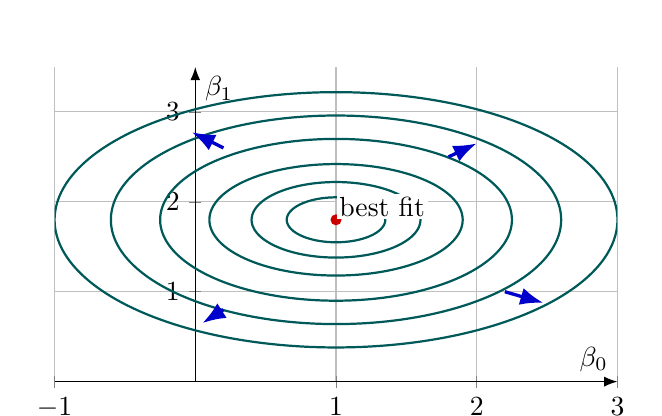
\begin{tikzpicture}
\begin{axis}[
  width=0.72\textwidth,
  height=0.46\textwidth,
  xmin=-1,xmax=3,
  ymin=0,ymax=3.5,
  axis lines=middle,
  xlabel={$\beta_0$},ylabel={$\beta_1$},
  grid=both,
  axis line style={-Latex}
]
\foreach \a/\b in {0.35/0.25,0.6/0.42,0.9/0.62,1.25/0.9,1.6/1.16,2.0/1.42}{
  \addplot[domain=0:360,samples=220,teal!70!black,thick] ({1.0 + \a*cos(x)},{1.8 + \b*sin(x)});
}
\fill[red!80!black] (axis cs:1.0,1.8) circle (2pt);
\node[above right,fill=white,inner sep=1pt] at (axis cs:1.0,1.8) {best fit};
\foreach \px/\py/\ux/\vy in {0.2/0.8/-0.6/-0.6,1.8/2.5/0.8/0.6,2.2/1.0/1.1/-0.5,0.2/2.6/-0.9/0.7}{
  \pgfmathsetmacro{\rx}{\px+0.25*\ux}
  \pgfmathsetmacro{\ry}{\py+0.25*\vy}
  \addplot[blue!80!black,very thick,-Latex] coordinates {(\px,\py) (\rx,\ry)};
}
\end{axis}
\end{tikzpicture}
\caption{The gradient of a least-squares loss points toward increasing loss; the negative gradient points downhill.}
\end{figure}

\section{Common mistakes}

\begin{warningbox}[Mistake 1: Differentiating every variable at once]
When computing $f_x$, only $x$ varies. All other variables are constants. For example, if $f(x,y)=x^2y$, then $f_x=2xy$, not $2xy+x^2$.
\end{warningbox}

\begin{warningbox}[Mistake 2: Confusing partial derivatives with total change]
The partial derivative $f_x(a,b)$ measures change only in the $x$ direction. It does not describe motion along an arbitrary path unless the path moves only in the $x$ direction.
\end{warningbox}

\begin{warningbox}[Mistake 3: Forgetting to normalize a direction vector]
In the directional derivative formula $D_u f=\grad f\cdot u$, the vector $u$ must be a unit vector. If a problem gives a nonunit direction vector, divide by its length first.
\end{warningbox}

\begin{warningbox}[Mistake 4: Assuming mixed partials are always equal]
Mixed partials are equal under hypotheses such as continuity near the point. For standard smooth examples this is usually true, but the theorem has a condition.
\end{warningbox}

\section{Chapter exercises}

\subsection*{Conceptual questions}
\begin{enumerate}
  \item Explain in words what $f_x(a,b)$ means.
  \item Explain why $f_x(a,b)$ is the slope of a trace of the surface $z=f(x,y)$.
  \item Explain the difference between $f_x(a,b)$ and $f_y(a,b)$.
  \item Why is a partial derivative not the same thing as a directional derivative in every direction?
  \item Explain why $\grad f$ is perpendicular to a level curve.
  \item In an image, what do large values of $|I_x|$ and $|I_y|$ usually indicate?
  \item In a loss function $L(\theta_1,\theta_2)$, what does $\partial L/\partial \theta_1$ mean?
  \item Explain why the gradient is useful even when the function has many variables.
\end{enumerate}

\subsection*{Skill problems}
\begin{enumerate}[start=9]
  \item Find $f_x$ and $f_y$ for $f(x,y)=x^2y+3xy^2-y$.
  \item Find $f_x$ and $f_y$ for $f(x,y)=e^{xy}+\ln(x+y)$ on its domain.
  \item Find $f_x$ and $f_y$ for $f(x,y)=\cos(x^2+y^2)$.
  \item Find $\grad f(1,2)$ for $f(x,y)=x^3y+y^2$.
  \item Find $\grad f(0,1)$ for $f(x,y)=\sin(xy)+e^y$.
  \item Find $\grad f(1,2,3)$ for $f(x,y,z)=x^2y+yz^3$.
  \item Find all four second partial derivatives of $f(x,y)=x^2+xy^3+\sin(xy)$.
  \item Verify Clairaut's theorem for $f(x,y)=e^{xy}+x^2y^3$.
  \item Estimate $f_x(2,1)$ using $f(2,1)=5.0$ and $f(2.1,1)=5.32$.
  \item Estimate $f_y(2,1)$ using $f(2,1)=5.0$ and $f(2,1.2)=4.7$.
\end{enumerate}

\subsection*{Applied and computational problems}
\begin{enumerate}[start=19]
  \item Let $H(x,y)=1100-2x^2-y^2$ model the height of a hill in meters. Compute $H_x$ and $H_y$, and interpret them.
  \item For the same hill, compute $\grad H(10,20)$ and explain what the signs of its components mean.
  \item Let $T(x,y,z)=xe^y+0.5z^2$. Compute $\grad T(1,0,3)$.
  \item Let $I$ be an image intensity function. Explain how finite differences approximate $I_x$ and $I_y$.
  \item For least-squares regression with two parameters, derive the gradient of
  \[
  L(\beta_0,\beta_1)=\sum_{i=1}^m \left(y_i-(\beta_0+\beta_1x_i)\right)^2.
  \]
  \item Write code to approximate $\grad f(1,2)$ for $f(x,y)=x^3+x^2\sin y-xe^y$ using centered differences.
  \item Generate a contour plot of $f(x,y)=x^2+4y^2$ and draw gradient vectors at several points.
  \item Compute numerical gradients on a grid for $f(x,y)=\sin x\cos y$.
\end{enumerate}

\subsection*{Challenge problems}
\begin{enumerate}[start=27]
  \item Let $f(x,y)=\sqrt{x^2+y^2}$. Show that $f_x(0,0)$ and $f_y(0,0)$ exist, but explain why this does not mean the surface has a tangent plane at the origin.
  \item Find a function for which $f_x$ and $f_y$ exist at the origin but the function is not continuous at the origin.
  \item Suppose $f(x,y)=g(x^2+y^2)$ for a differentiable single-variable function $g$. Find $\grad f$.
  \item Suppose $f(x,y)=h(ax+by)$ for a differentiable single-variable function $h$. Find $\grad f$ and describe the direction of the gradient.
  \item Let $f(x,y,z)=F(x^2+y^2+z^2)$. Find $\grad f$ and describe its direction geometrically.
  \item In a high-dimensional model, the gradient has one component per parameter. Explain why this makes gradient methods scalable compared with searching every direction separately.
\end{enumerate}

\section{Python lab and interactive page}

The Python lab for this chapter focuses on numerical and visual differentiation:
\begin{itemize}
  \item estimating partial derivatives from function values;
  \item comparing forward, backward, and centered differences;
  \item plotting coordinate traces of surfaces;
  \item visualizing gradients on contour plots;
  \item computing image gradients;
  \item computing gradients of least-squares losses.
\end{itemize}

Resources:
\begin{itemize}
  \item Chapter 8 Python lab: \texttt{../labs/Chapter08\_Partial\_Derivatives\_and\_the\_Gradient.ipynb}
  \item Chapter 8 interactive HTML page: \texttt{../htmls/chapter-08.html}
\end{itemize}

\section{Chapter summary}

Partial derivatives are the coordinate-direction derivatives of a multivariable function. They are ordinary derivatives applied to slices of the function. For $f(x,y)$, the two first partial derivatives are $f_x$ and $f_y$. For a function of $n$ variables, there are $n$ first partial derivatives.

The gradient packages these partial derivatives into a vector:
\[
\grad f=\left\langle
\frac{\partial f}{\partial x_1},
\ldots,
\frac{\partial f}{\partial x_n}
\right\rangle.
\]
This vector is perpendicular to level sets and contains the first-order sensitivity information of the function. In modern applications, the gradient is the basic object behind numerical differentiation, image processing, optimization, maximum likelihood, backpropagation, and gradient-based learning.

\end{document}
